\section{Finite Markov Decision Processes}

This chapter introduces the formal definition of Markov Decision Processes and the optimal policies.

\subsection{The Agent-Environment Interface}

The MDP is a mathematical framework for modeling decision-making problems. It formulates the problem as an agent interacting with an environment. The agent and the environment interact at discrete time steps, and the agent makes decisions based on the environment's state. The environment then transitions to a new state, and the agent receives a reward based on the transition.

\begin{figure}[h!]
    \centering
    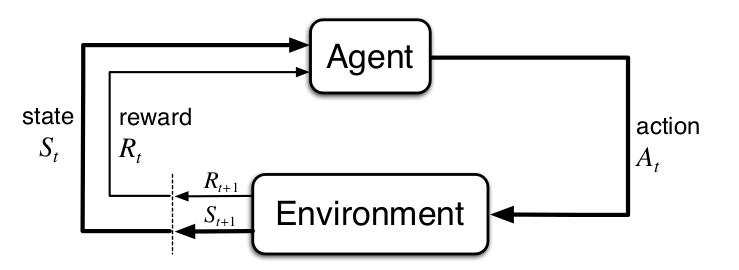
\includegraphics[width=0.7\textwidth]{images/agent-environment.png}
    \caption{The agent-environment interface in a Markov Decision Process.}
    \label{fig:agent-environment}
\end{figure}

The interactions between the agent and the environment are taken to be at a sequence of discrete time steps $t=0,1,2,3,\dots$. At each time step $t$, the agent receives some representation of the environment's state $S_t \in \mathcal{S}$, where $\mathcal{S}$ is the set of all possible states. The agent then selects an action $A_t \in \mathcal{A}(S_t)$, where $\mathcal{A}(S_t)$ is the set of all possible actions in state $S_t$. The environment then transitions to a new state $S_{t+1}$ and the agent receives a reward $R_{t+1}\in\mathcal{R}\subset\mathbb{R}$. The agent's goal is to maximize the cumulative reward it receives over time. The MDP and agent together give rise to a sequence or \textit{trajectory} that is a sequence of state-action-reward triples.

\begin{equation}
    S_0, A_0, R_1, S_1, A_1, R_2, S_2, A_2, R_3, S_3, A_3, R_4, \dots
\end{equation}

In a finite MDP, the sets of states, actions, and rewards are all finite. The agent-environment interface in a finite MDP is shown in Figure~\ref{fig:agent-environment}. The random variables $R_t$ and $S_t$, have a well-defined probability distribution that depends only on the preceding state and action. That is for particular values of these random variables $s'\in\mathcal{S}$ and $r\in\mathcal{R}$, there is a probability of these values occurring given the preceding state and action:\begin{equation}
    p(s',r \mid s,a) \doteq \text{Pr}\{S_t=s', R_t=r \mid S_{t-1}=s, A_{t-1}=a\}
\end{equation}for all $s',s\in\mathcal{S}, r\in\mathcal{R}$ and $a\in\mathcal{A}(s)$

\begin{equation}
    \sum_{s'\in\mathcal{S}}\sum_{r\in\mathcal{R}}p(s',r \mid s,a) = 1 \text{ for all } s\in\mathcal{S}, a\in\mathcal{A}(s)
\end{equation}

If a state $s'$ and reward $r$ depend only on the preceding state and action, then the environment is said to be a \textit{Markov Decision Process}. And, if a state contains all relevant information from the history, then the state is said to be \textit{Markov} and the process is said to have the \textit{Markov Property}.

\begin{equation}
    p(s' \mid s,a) \doteq \text{Pr}\{S_t=s' \mid S_{t-1}=s, A_{t-1}=a\} = \sum_{r\in\mathcal{R}}p(s',r \mid s,a)
\end{equation}
\begin{equation}
    r(s,a) \doteq \mathbb{E}[R_t \mid S_{t-1}=s, A_{t-1}=a] = \sum_{r\in\mathcal{R}}r\sum_{s'\in\mathcal{S}}rp(s',r \mid s,a)
\end{equation}

The goal of any agent is to maximize its rewards.

\subsection{Returns and Episodes}

The agent run can be taken as \textit{continuing} or \textit{episodic}, to consider the iterations of the game.

For example, consider a robot that is trying to navigate a maze. In the continuing case, the robot continues to navigate the maze indefinitely, and the agent-environment interaction does not terminate. In the episodic case, the robot navigation is considered as episodes of trying to reach the goal and an episode ends when the robot reaches the goal or when it gets stuck in the maze.

\textit{Continuing} method is used when the life of the bot is long and needs to survive, while \textit{Episodic} is used to define short games.

The agent tries to maximize the cumulative reward it receives over time. The \textit{expected return}\begin{equation}
    G_t \doteq R_{t+1} + R_{t+2} + R_{t+3} + \dots + R_T
\end{equation} where the $T$ is the final time step of the episode. The return depends on the rewards received by the agent at each time step. The agent's goal is to maximize the expected return over time.

When the life-span is not finite, the $G_t$ doesn't converge as $T\rightarrow \infty$. Hence, a factor of $\gamma$ is used to define $G_t$ as
\begin{align*}
    G_t &\doteq R_{t+1} + \gamma R_{t+2} + \gamma^2 R_{t+3} + \gamma^3 R_{t+4} + \dots \\
    &= R_{t+1} + \gamma(R_{t+2} + \gamma R_{t+3} + \gamma^2 R_{t+4} + \dots) \\
    &= R_{t+1} + \gamma G_{t+1}
\end{align*}

This even works even when termination occurs at $t=T$, provided we define $G_T=0$.

\subsection{Policies and Value Functions}

A \textit{policy} is a mapping from states to probabilities of selecting each possible action. If an agent is following a policy $\pi$ at a time, the probability of choosing an action $a$, when you're in the state $s$ is denoted by $\pi(a \mid s)$.

The \textit{value function} of a state $s$ under a policy $\pi$, denoted by $v_\pi(s)$, is the expected return when starting in s, following the policy $\pi$.

\begin{equation}
    v_\pi(s) \doteq \mathbb{E}_\pi\left[G_t\mid S_t=s\right] = \mathbb{E}_\pi\left[\sum_{k=0}^{\infty}\gamma^{k}R_{t+k+1} \biggm| S_t=s\right]
\end{equation}

The expected return when we choose an action $a$ from $s$, following the policy $\pi$, is defined as $q_\pi(s, a)$ and is defined as

\begin{equation}
    q_\pi(s, a) \doteq \mathbb{E}_\pi\left[G_t\mid S_t=s, A_t=a\right] = \mathbb{E}_\pi\left[\sum_{k=0}^{\infty}\gamma^{k}R_{t+k+1} \biggm| S_t=s, A_t=a\right]
\end{equation}

\begin{align}
    v_\pi(s) &\doteq \mathbb{E}_\pi\left[G_t\mid S_t=s\right] \\
    &= \mathbb{E}_\pi\left[R_{t+1} + \gamma G_{t+1} \mid S_t=s\right] \\
    &= \sum_{a}\pi(a\mid s)\sum_{s',r}p(s',r\mid s,a)\left[r + \gamma\mathbb{E}_\pi\left[G_{t+1}\mid S_{t+1}=s'\right]\right] \\
    &= \sum_{a}\pi(a\mid s)\sum_{s',r}p(s',r\mid s,a)\left[r + \gamma v_\pi(s')\right], \quad \text{for all } s\in\mathcal{S}\label{eq:bellman-v}
\end{align}

The equation~\ref{eq:bellman-v} is called the \textit{Bellman Equation} for $v_\pi$. It expresses a relationship between the value of a state and the values of its successor states.

\subsection{Optimal Policies and Optimal Value Functions}

The goal of Reinforcement Learning is to find the optimal policy $\pi$, which maximizes the expected return. A policy $\pi$ is defined to be better than or equal to another policy $\pi'$ if $v_\pi(s) \geq v_{\pi'}(s)$ for all $s\in\mathcal{S}$. In other words, $\pi \geq \pi'$ if and only if $v_\pi(s) \geq v_{\pi'}(s)$ for all $s\in\mathcal{S}$. The optimal policy is denoted by $\pi_\ast$. The optimal value function is denoted by $v_\ast$ and is defined as\begin{equation}
    v_\ast(s) \doteq \max_\pi v_\pi(s)
\end{equation} for all $s\in\mathcal{S}$ and the optimal action-value function is defined as\begin{equation}
    q_\ast(s, a) \doteq \max_\pi q_\pi(s, a)
\end{equation} for all $s\in\mathcal{S}$ and $a\in\mathcal{A}(s)$.

The optimal value function satisfies the Bellman Optimality Equation, which is given by\begin{equation}
    v_\ast(s) = \max_a\sum_{s',r}p(s',r\mid s,a)\left[r + \gamma v_\ast(s')\right]
\end{equation} for all $s\in\mathcal{S}$. The optimal action-value function satisfies the Bellman Optimality Equation, which is given by\begin{equation}
    q_\ast(s, a) = \sum_{s',r}p(s',r\mid s,a)\left[r + \gamma\max_{a'}q_\ast(s', a')\right]
\end{equation} for all $s\in\mathcal{S}$ and $a\in\mathcal{A}(s)$.

The Bellman Optimality Equation is a recursive equation and applying this equation gives simultanious nonlinear equations, which when solved gives the best optimal policy. But solving the Bellman Optimality Equation is computationally expensive and infeasible for large MDPs. Hence, we use iterative methods to solve the Bellman Optimality Equation.
